%%%%%%%%%%%%%%%%%%%% book.tex %%%%%%%%%%%%%%%%%%%%%%%%%%%%%
%
% sample root file for the chapters of your "monograph"
%
% Use this file as a template for your own input.
%
%%%%%%%%%%%%%%%% Springer-Verlag %%%%%%%%%%%%%%%%%%%%%%%%%%


% RECOMMENDED %%%%%%%%%%%%%%%%%%%%%%%%%%%%%%%%%%%%%%%%%%%%%%%%%%%
\documentclass[envcountsame,envcountchap]{svmono}
%\documentclass[envcountsame,envcountchap]{svmono}

% choose options for [] as required from the list
% in the Reference Guide, Sect. 2.2

\usepackage{makeidx}         % allows index generation
\usepackage{graphicx}        % standard LaTeX graphics tool
\usepackage{amsmath,amssymb}         % matrices
\usepackage{enumerate}
                             % when including figure files
\usepackage{multicol}        % used for the two-column index
\usepackage[bottom]{footmisc}% places footnotes at page bottom
% etc.
% see the list of further useful packages
% in the Reference Guide, Sects. 2.3, 3.1-3.3


\DeclareMathOperator{\End}{End}
\DeclareMathOperator{\Aut}{Aut}
\DeclareMathOperator{\Hom}{Hom}
\DeclareMathOperator{\support}{supp}


% NEW COMMANDS

%It is standard in Latex to write "macros" which are shorthand for an entire series of instructions. Here are some examples

%Number sets
\newcommand{\N}{\mathbb N}
%So typing \N produces the correct mathematical symbol for the natural numbers
\newcommand{\Z}{\mathbb Z}
\newcommand{\Q}{\mathbb Q}
\newcommand{\R}{\mathbb R}
\newcommand{\C}{\mathbb C}
\newcommand{\K}{\mathbb K}
%notations quelquonques
\newcommand{\tg}[1]{\textbf{#1}}
\newcommand{\ub}[1]{\overline{#1}}

%notations des objets simples
\newcommand{\es}{\emptyset}
\newcommand{\nes}{$\not= \emptyset$}
\newcommand{\sub}{\subset}
\newcommand{\norm}[2]{\lVert #1 \lVert_{#2}}
\newcommand{\vect}[2]{(#1_1,#1_2, \dots, #1_#2)}
\newcommand{\modu}[1]{\lvert#1\lvert}
\newcommand{\B}[3]{B_{#1}\big(#2,#3\big[}
%notations mathématiques
\newcommand{\lb}{\lbrack}
\newcommand{\rb}{\rbrack}
\newcommand{\lv}{\lVert}
%limits and sum
\newcommand{\s}[2]{\sum\limits_{#1}^{#2}}
\newcommand{\li}[2]{\xrightarrow[#1\rightarrow#2]{}}
\newcommand{\lis}[1]{\xrightarrow[n\rightarrow+\infty]{#1}}
\newcommand{\lif}[1]{\xrightharpoonup[n\rightarrow+\infty]{#1}}
\newcommand{\lic}[3]{\xrightarrow[#1\rightarrow#2]{#3}}

\newcommand{\bcup}[2]{\bigcup\limits_{#1}^{#2}}
\newcommand{\bcap}[2]{\bigcap\limits_{#1}^{#2}}

\newcommand{\inv}[1]{\frac{1}{#1}}
\newcommand{\prods}[2]{\langle\qq #1\qq,\qq#2\qq\rangle}

\newcommand{\restr}[2]{#1_{\mkern 2mu \vrule height 2ex\mkern2mu #2} }
\newcommand{\quot}[2]{{\raisebox{.2em}{$#1$}\left/\raisebox{-.2em}{$#2$}\right.}}
\newcommand{\limite}[2]{\underset{#1\rightarrow#2}{\text{lim}}}
\newcommand{\espp}[2]{Ker\big(u-{#1} Id_{#2}\big)}
\newcommand{\fct}[4]{\qq:\qq #1\qq\longrightarrow\qq #2\qq :\qq #3\qq \mapsto\qq #4}

\newcommand{\lam}{\lambda}
\newcommand{\q}{\quad}
\newcommand{\qq}{\text{ }}

\newcommand{\liste}[2]{#1_1, #1_2,..,#1_{#2}}

\newcommand{\maxx}[1]{\underset{#1}{\text{max}}}
\newcommand{\minn}[1]{\underset{#1}{\text{min}}}
\newcommand{\supp}[1]{\underset{#1}{\text{sup}}}
\newcommand{\inff}[1]{\underset{#1}{\text{inf}}}

\newcommand{\fctt}[2]{\qq:\qq#1\qq\rightarrow\qq#2}
\newcommand{\liminff}[1]{\underset{#1\rightarrow+\infty}{\text{liminf}}}
\newcommand{\limsupp}[1]{\underset{#1\rightarrow+\infty}{\text{limsup}}}

\newcommand{\adh}[2]{\text{Adh}_{#1}\big(#2\big)}
\newcommand{\wed}[3]{#1_#2\wedge\dots \wedge #1_#3}


\makeindex             % used for the subject index
                       % please use the style svind.ist with
                       % your makeindex program


%%%%%%%%%%%%%%%%%%%%%%%%%%%%%%%%%%%%%%%%%%%%%%%%%%%%%%%%%%%%%%%%%%%%%

\begin{document}

\author{MATH-F-427 students}
\title{Coxeter groups}
\subtitle{Course notes}
\maketitle

\frontmatter%%%%%%%%%%%%%%%%%%%%%%%%%%%%%%%%%%%%%%%%%%%%%%%%%%%%%%

\tableofcontents


\mainmatter%%%%%%%%%%%%%%%%%%%%%%%%%%%%%%%%%%%%%%%%%%%%%%%%%%%%%%%
\part{Coxeter groups}

\section{Parabolic subgroup and parabolic quotient.}
The last ingredient needed to study the link between Coxeter groups and geometry is the notions of Parabolic subgroup and Parabolic quotient. The purpose of this section is to define those two and to investigate some of their basic properties.

\begin{definition}
	Let $(W,S)$ be a Coxeter system and let $J$ be a subset of $S$ then, we define the \tg{parabolic subgroup} of $W$ associated to $J$ as the group generated by $J$ :
	\begin{equation}
	W_J\qq=\qq <\qq J\qq >\qq \sub \qq W
	\end{equation} 
\end{definition}
\begin{remark}
	Before going further, let us remark that for any non empty subset $J\sub S$, the pair $(W_J,J)$ defines a Coxeter system, since it just restrict the set of generators without changing their intertwining relations. We will discuss the proof of this fact in more detail in the next proposition.
\end{remark}
\begin{example}
	Let us consider the Coxeter group $S_7$ together with its set of generators  $S=\{s_1,s_2,\dots, s_6\}$ and its classical presentation. If we consider the subset $J=\{s_1,s_2,s_3,s_5,s_6\}$. then, the associated parabolic group is :
	\begin{equation}
	W_J\qq=\qq <\qq <\{s_1,s_2,s_3\}>\qq \cup \qq <\{s_5,s_6\}>\qq >\qq \simeq\qq S_4\qq \times \qq S_3
	\end{equation}
\end{example}
In fact, the phenomena observed in the latest is a general fact when it comes to the symmetric group $S_n$. Namely, if we take any partition of $n$, meaning any multi index $\alpha=(\alpha_1,\alpha_2,\dots, \alpha_k)$ such that $\s{i=1}{k}\alpha_i=n$, $\alpha_i\in \N\backslash\{0\}$ and if we consider $J$ as the set containing the $s_i$ for $i\in \lb \alpha_{2j},\alpha_{2j+1}\rb$ for every $j\in \N$ such that $2j\leq n$. We have that :
\begin{equation}
S_\alpha\qq=\qq S_{\alpha_1}\times S_{\alpha_3}\times \dots \times S_{\alpha_{2k+1}}
\end{equation}
Where $2k+1$ is the bigger odd index less or equal than $n$.

The following proposition investigate some properties of this parabolic group associated to $J$.
\begin{proposition}
	Le $(W,S)$ be a Coxeter system and let $I,J$ be two subsets of $S$. Then, the following properties holds :
	\begin{enumerate}
		\item The pair $(W_J,J)$ defines a Coxeter system.
		\item If we denote by $l_J$ the length of a coefficient then for every $w\in W_J\sub W$ we have that :
		\begin{equation}
		l_J(w)\qq=\qq l(w)
		\end{equation} 
		\item\begin{center}
			$W_I\cap W_J=W_{I\cap J}$
		\end{center}
		\item \begin{center}
			$<\qq W_I\cup W_J\qq >\qq=\qq W_{I\cap J}$
		\end{center}
		\item\begin{center}
			 $W_I=W_J\qq \iff \qq I=J$
		\end{center}
	\end{enumerate} 
\end{proposition}
\begin{proof}
	We are going to prove each point separately :
	\begin{enumerate}
		\item Using Matsumata's Theorem, we know that it is enough to prove that the deletion property holds in $(W_J,J)$. But every element of $W_J$ is in particular an element of $W$. Since the deletion property holds in the $W$, we can apply it on the element $w$ and we proved that the deletion property still holds in $(W_J,J)$, which proves it's a Coxeter system.
		\item Let us take $w\in W_J$ and let us right $w=j_1j_2...j_r$ for some $j_i\in J$ and $r=l_J(w)$. Since $w$ is an element of $W$ and $J$ is a subset of $S$ we deduce that $l(w)\leq r$ because our last writing of $w$ in $(W_J,J)$ is also a writing of $w$ in $(W,S)$. Now, let us suppose by absurd that $l(w)\not=l_J(w)$, this means that $l(w)<r$. In particular, this means that we can find by deletion property a subword of $w$ in $(W,S)$ but, since $w$ was written only with element of $J$, this subword contains only elements of $J$. Therefore, we also reduced the word $w$ in $(W_J,J)$ which is a contradiction with the fact that $r=l_J(w)$.
		\item We prove this equality in two inclusions. the inclusion $W_{I\cap J}\sub W_I\cap W_J $ is clear from the definition of group generated by a set. Now let us show the opposite inclusion. Let $w\in W_I\cap W_J$ and let $j_1j_2...j_q=w=i_1i_2...i_q$ be two reduced writing of $w$ in $(W_J,J)$ and $(W_I,I)$ respectively (let us remark that we can write it as the product of $q$ elements in both $J$ and $I$ because of the first second point of the proposition which asserts that $l_J(w)=l(w)=l_I(w)$). Since the equality of the two writings hold in $W$ and since we already saw as a consequence of the deletion property that two reduced writing of $w$ in $(W,S)$ are made with the same set of element we obtain that as a sets :$\{i_1,...,i_r\}=\{j_1,...j_r\}$ therefore, we deduce that $\{i_1,...,i_r\}=\{j_1,...j_r\}\sub I\cap J$ and $w$ is in the subgroup generated by $I\cap J$.
		\item This point is clear since it is true for any subsets $I,J$ of a group $W$ that the union of the group generated by $I$ and $J$ respectively is the group generated by the union $I\cup J$.
		\item The implication $(\Leftarrow)$ is obvious. When it comes to the implication $(\Rightarrow)$, let us suppose by absurd that $I\not=J$ and let us take any $i\in I\backslash J$. Since $i\in I\sub W_I=W_J$ we obtain that $i$ can be written in terms of element of $J$ and since $i$ is a reduced word this means that $i$ can be written in terms of elements of $J$ with only one element $j$. Further more, as a consequence of the deletion property we know that $\{i\}=\{j\}$ and therefore $i=j\in J$ which is a contradiction.
	\end{enumerate}
\end{proof}
\begin{definition}
	Let $(W,S)$ be a Coxeter system and let $J\sub S$ then, we define its parabolic quotient as the space :
	\begin{equation}
	W^J\qq=\qq\{w\in W\qq \lvert\qq wj>w\qq \mbox{for all }j\in J\}
	\end{equation}
\end{definition}

As we will see later, this parabolic quotient $W^J$ associated to $J$ is a set containing every of the left coset representatives of the parabolic subgroup $W_J$ in $W$. Unfortunately, this parabolic quotient is usually not a group.

	
The following proposition gives a second point of view of this parabolic quotient :
\begin{proposition}
	Let $(W,S)$ be a Coxeter system and let $J\sub S$ then :
	\begin{equation}
	W^J\qq=\qq\{w\in W\qq :\qq \mbox{no reduced critting of } w \mbox{ ends with an element of }J\}
	\end{equation}
\end{proposition}
\begin{proof}
	We are going to show that the complementary of $W^J$ is the complementary of the above set. Now, to show this set equality we are going to prove two inclusions. The inclusion $\supset$ is clear. Indeed, if a reduced word of $w$ end up with an element $j\in J$ then $l(wj)=l(w)-1$ and therefore, $l(wj)<l(w)$ which proves that $w\in (W^J)^c$. The proof the second inclusion is a straightforward consequence of the exchange property. Indeed, let $w\in (W^J)^c$, and let us consider a writing of $w=s_1...s_k$ such that it is a reduced word of $W$. Since $w\in (W^J)^c$ we know that $wj\leq w$ for some $j\in J$. By an argument of parity since $J\sub S$ the only possibility is that $l(wj)<l(w)$. But, since $J\sub S\sub T$ we can apply the exchange property and we obtain that $wj=s_1...s_{i-1}\check{s_i}s_{i+1}...s_k$ for some index $i\in \{1,2,...,k\}$. In particular, since $j\in J\sub S$, the only possibility it that $i=k$ and that $s_k=j$ otherwise, we would lose more that only one index in the writing of $wj$. Therefore, the reduced writing of $w$ ended with an element of $j\in J$. \qed
\end{proof}
Now, let us consider an explicit example of parabolic subgroup and quotient that will be associated. Let us consider the Coxeter system $(S_3,\{s_1,s_2\})$ and the set $J=\{s_1\}$. Then the associated parabolic subgroup is $W_J=\{e,s_1\}$ and the associated parabolic quotient is $W^J=\{e,s_2,s_1s_2\}$. The following figure represent the Bruhat diagram of this Coxeter group and give a good intuition of why $W^J$ should be the set of representatives for the coset of $W_J$ in $W$.
\begin{figure}[h]
		\centering
		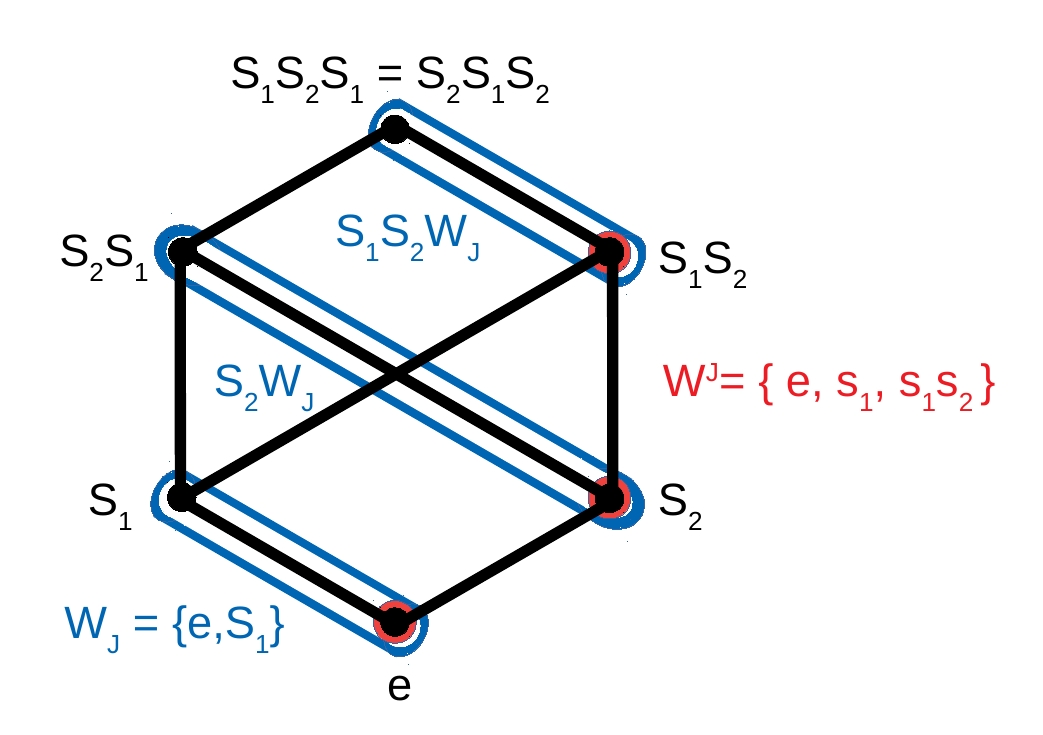
\includegraphics[scale=0.2]{Coxetergroupimagediamand.JPG}
\end{figure}

\begin{proposition}
	Let $(W,S)$ be a Coxeter system, and let $J\sub S$ be a non empty subset of $S$. Then, every element $w\in W$ factors uniquely as a product $w=w^Jw_J$ of an element $w_J$ of the parabolic subgroup $W_J$ and an element $w^J$ of the parabolic quotient $W^J$. Furthermore, $l(w)=l(w_J)+l(w^J)$.
\end{proposition}
\begin{proof}
	Start with a reduced $w$. There is two cases. Either there exists no $j\in J$ such that $w>wj$ and $w\in W^J$ which implies that $w=w\qq e\in w^JW_J$ and we are done. Or there exist some $j_1\in J$ such that $w>wj_1$. In that last case, we can repeat the process. Either there exists no $j\in J$ such that $wj_1>wj_1j$ and $wj_1\in W^J$ therefore $w=wj_1\qq j_1\in w^JW_J$ and we are done. Or there exist some $j_2\in J$ such that $wj_1>wj_1j_2$. In that case, we can again repeat the process. However, this process need to stop at some point since there is a finite number of letters in any reduced writing of $w$ and since each time a relation $>$ occurs the word becomes at least one letter shorter. In particular, we obtain a sequence :
	\begin{equation}
	w\qq >\qq wj_1\qq >wj_1j_2\qq >\qq ...\qq >\qq wj_1...j_k
	\end{equation}
	for some $k\in\N$ with $k<l(w)$ and some $j_1,...,j_k\in J$, such that $wj_1...j_k\in W^J$. Therefore, we can write $w=wj_1...j_k\qq j_k...j_1\in W^JW_J$ and we obtain what we wanted. Furthermore, since from this process, we observe that $l(wj_1...j_k)=l(w)-k$ we obtain that $l(wj_1...j_k)+l(j_1...j_k)\qq\leq \qq l(w)-k+k=l(w)$. And since $w=w^Jw_J$ we had the opposite inequality $l(w)\leq l(w^J)+l(w_J)$. Therefore, we conclude that $l(w)=l(w^J)+l(w_J)$.  
	
	Now, we need to prove that this decomposition is unique. let us suppose that $w=w^Jw_J=v^Jv_J$ for some $w^J,v^J\in W^J$ and some $w_J,v_J\in W_J$. Then, $w^J=v^J\qq v_Jw_{J}^{-1}$ and since $W_J$ form a group, we deduce that $v_Jw_{J}^{-1}\in W_J$. Now, chose some reduce writing for $v^J$ in $W$ and some reduce writing for $v_Jw_J^{-1}$ in $W_J$. By deletion, we know that we can reduce the obtained writing of the word $w^J=v^J\qq v_Jw_{J}^{-1}$ and since this reduced word belongs to $W^J$ we know that it can't end with an element of $J$. Therefore, $w^J$ must be a subword of $v^J$. In particular, $w^J\leq v^J$ and by symmetry, using the same reasoning, we will obtain that $v^J\leq w^J$ from which we conclude that $w^J=v^J$ and therefore that $vw_J=v_J$. Thus, the decomposition must be unique.
\end{proof}
A simple but very important corollary of this proposition is, as announced before, that the parabolic quotient gives a complete set of representatives for the left cosets of $W_J$. Furthermore, we have the following :
\begin{corollary}
	The left coset $wW_J$ of $W_J$ in $W$ has a unique minimal element. Further more, this unique minimal element of $wW_J$ is precisely the element $w^J$ appearing in the decomposition of $w=w^Jw_J$. 
\end{corollary}
\begin{proof}
	From the decomposition of $w$ given by $w=w^Jw_J$ it is clear that $w^J=ww_J^{-1}\in wW_J$. Now, our task is to show that this is a minimal element of $wW_J$ for the Bruhat order. Following this purpose, let $v\in W_J$ and let us consider the element $wv\in wW_J$. Then, we have that :
	\begin{equation}
	wv\qq=\qq w^J\qq w_Jv,
	\end{equation}
	with $w_Jv\in W_J$. Therefore, by unicity of the factorisation of $w$ as a product in $W^JW_J$ we obtain that $(wv)_J=  w_Jv$. Therefore we have that :
	\begin{equation}
	l(wv)\qq=\qq l(w^J)\qq+\qq l(w_Jv)\qq \geq \qq l(w^J)
	\end{equation}
	which prove that no other element of $wW_J$ can be smaller than $w^J$ for the Burhat order. In particular, $w^J$ is minimal in the coset $wW_J$. Now, we need to prove that it is the unique minimal element of this coset. Now, let us take any $wv\in wW_J$. We know that the decomposition $wv=w^J\qq w_Jv$ is unique. Therefore, if had considered a reduced writing of $wv$ and since $l(wv)\qq=\qq l(w^J)\qq+\qq l(w_Jv)$, we see that the reduced $w^J$ is a subword of the reduced $wv$ and is therefore comparable for the Burhat order with $w^J$. In particular, we obtain that $w^J\leq wv$ which proves that $w^J$ is the unique minimal element of $wW_J$.
\end{proof}
As always, let $(W,S)$ be a Coxeter system and let us consider a subset $J\sub S$. We are going to investigate some properties of the projection :
\begin{equation}
P_J\fct{W}{W^J}{w}{w^J}
\end{equation} 
\begin{proposition}
	The projection $P_J$ is order preserving for the Burhat order on $W$. This means that if $w_1\leq w_2$ for some elements $w_1,w_2\in W$ then $P_J(w_1)=w_1^J\leq w_2^J=P_J(w_2)$.
\end{proposition}
\begin{proof}
	This proposition is proved by induction on the length of $w_2$. For $l(w_1)=l(w_2)$, since $w_1\leq w_2$, the only possibility is that $w_1=w_2$ and therefore,  $w_1^J=w_2^J$. In particular, this proves that $P_J(w_1)\leq P_J(w_2)$.
	
	If now $w_1<w_2$ then, we know that $w_1^J\in w_1W_J$ and $w_1^J\leq w_1$. Therefore, if $w_2^J=w_2$ we are done since $w_1^J\leq w_1<w_2=w_2^J$. On the contrary, if $w_2\not=w_2^J$, then $w_2 > w_2^J$. Furthermore, since $w_2\not\in W^J$ there exists a $j\in J$ such that $w_2j\leq w_2$. But by definition of $W^J$ we have that $w_1^Jj>w_1^J$ and therefore we can apply the lifting property to the four elements : $w_2j, w_2, w_1, w_1j$ and we obtain that $w_1^J\leq w_2j < w_2$ Therefore, $w_1^J$ and $w_2j$ are two comparable elements such that $w_1^J\leq w_2j$ and since there length is less than the one of $w_2$ they respect the induction hypothesis and we therefore obtain that :
	\begin{equation}
	P_J(w_1)=w_1^J\qq=\qq P_J(w_1^J)\qq\leq \qq P_J(w_2 j)\qq=\qq w_2^J=P_J(w_2)
	\end{equation}
	and the proposition is proved.
\end{proof}

\section{Some geometry : The root systems.}
Let $V$ be a finite dimensional vector space over $\R$ and let us pick some symmetric bilinear form $\prods{}{}$ on $V$.
\begin{definition}
	An element $\alpha$ of $V$ is \tg{isotropic} when $\prods{\alpha}{\alpha}\not=0$. 
\end{definition}
Any \tg{non}-isotropic element $\alpha\in V$ can be associated to some ``reflexion" on the vector space $V$ :
\begin{equation}
\sigma_\alpha(v)\qq=\qq v\qq -\qq 2\qq \frac{\prods{v}{\alpha}}{\prods{\alpha}{\alpha}}\qq\alpha
\end{equation}
It is not hard to realise that when $\prods{}{}$ is positive definite, those $\sigma_\alpha$ defines a honest reflections through the hyperplane perpendicular to $\alpha$.

The following proposition gives us some insight about what $\sigma_\alpha$ does as a linear transformation on the vector space $V$ :
\begin{proposition}\label{les sigma definisse une isometrie.}
	Let $V$ be a vector space equipped with a bilinear form $\prods{}{}$ then the linear application on $v$ given by $\sigma_\alpha$ respects the following :
	\begin{enumerate}
		\item The application $\sigma_\alpha$ is an involution. This means that \begin{equation}
		\sigma^2_\alpha\qq =\qq \mbox{Id}_V
		\end{equation}
		 In particular, this implies that $\sigma_\alpha \in \mbox{GL}(V)$.
		\item The application $\sigma_\alpha$ is an isometry for the bilinear form $\prods{}{}$. In other words, for every vectors $u,v\in V$ we have :
		\begin{equation}
		\prods{\sigma_\alpha(u)}{\sigma_\alpha(v)}\qq=\qq \prods{u}{v}
		\end{equation} 
		\item $\sigma_\alpha(\alpha)=-\alpha$
	\end{enumerate} 
\end{proposition}
\begin{proof}
	The proof is a straightforward computation in the three cases :
	\begin{enumerate}
		\item Let $v\in V$ and let us compute :
		\begin{equation}
		\begin{split}
		\sigma_\alpha\circ\sigma_\alpha(v)\qq&=\qq \sigma_\alpha(v)\qq -\qq 2\qq \frac{\prods{\sigma_\alpha(v)}{\alpha}}{\prods{\alpha}{\alpha}}\qq\alpha\\
		&=\qq  v\qq -\qq 2\qq \frac{\prods{v}{\alpha}}{\prods{\alpha}{\alpha}}\qq\alpha \qq -\qq \qq 2\qq \frac{\prods{v\qq -\qq 2\qq \frac{\prods{v}{\alpha}}{\prods{\alpha}{\alpha}}\qq\alpha}{\alpha}}{\prods{\alpha}{\alpha}}\qq\alpha\\
		&=\qq  v\qq -\qq 2\qq \frac{\prods{v}{\alpha}}{\prods{\alpha}{\alpha}}\qq\alpha \qq-\qq 2\qq \frac{\prods{v}{\alpha}}{\prods{\alpha}{\alpha}}\qq\alpha \qq+\qq 4 \qq \frac{\prods{v}{\alpha}}{\prods{\alpha}{\alpha}} \qq \frac{\prods{\alpha}{\alpha}}{\prods{\alpha}{\alpha}}\alpha\\
		&=\qq v
		\end{split}
		\end{equation}
		\item For every $u,v\in V$ we have that :
		\begin{equation}
		\begin{split}
		\prods{\sigma_\alpha(u)}{\sigma_\alpha(v)}\qq&=\qq\prods{ u\qq -\qq 2\qq \frac{\prods{u}{\alpha}}{\prods{\alpha}{\alpha}}\qq\alpha}{ v\qq -\qq 2\qq \frac{\prods{v}{\alpha}}{\prods{\alpha}{\alpha}}\qq\alpha}\\
		&=\qq\prods{u}{v}\qq-\qq 2  \frac{\prods{u}{\alpha}}{\prods{\alpha}{\alpha}} \prods{\alpha}{v}\qq -\qq 2 \frac{\prods{v}{\alpha}}{\prods{\alpha}{\alpha}}\prods{u}{\alpha}\\
		&\qq +\qq 4\qq \frac{\prods{u}{\alpha}}{\prods{\alpha}{\alpha}}\frac{\prods{v}{\alpha}}{\prods{\alpha}{\alpha}}\prods{\alpha}{\alpha}\\
		&=\qq \prods{u}{v}
		\end{split}
		\end{equation}
		\item Finally :
		\begin{equation}
		\sigma_\alpha(\alpha)\qq=\qq \alpha\qq -\qq 2\qq \frac{\prods{\alpha}{\alpha}}{\prods{\alpha}{\alpha}}\qq\alpha\qq=\qq \alpha\qq -\qq 2 \alpha\qq=\qq -\alpha
		\end{equation}
	\end{enumerate}
\end{proof}
Now, let us introduce the main definition of root system in a vector space $V$ equipped with some bilinear form $\prods{}{}$.
\begin{definition}
	A root system $(\Phi,\Delta)$ is a pair of two subsets of $V$ namely $\Phi$ the set of roots and $\Delta$ the set of simple roots. Such that $\Delta\sub \Phi\sub V$ with :
	\begin{enumerate}[({R}1)]
		\item For every simple root $\alpha\in \Delta$ we have $\prods{\alpha}{\alpha}>0$.
		\item The set of simple root $\Delta$ is a basis of $V$.
		\item If the multiple of a root by a real number is still a root then this real number is either $1$ or $-1$. Namely, if $\beta$ and $c\beta\in \Phi$ for some $c\in \R$ then either $c=1$ or $c=-1$.
		\item $\Phi=W\Delta$ where $W\qq=\qq <\{\sigma_\alpha\qq \lvert\qq \alpha\in \Delta\}>$.
		\item If $\beta\in \Phi$, then $\beta$ or $-\beta\in \R_{\geq 0}\Delta:=\Phi^+$ where the set $\R_{\geq 0}\Delta:=\Phi^+$ denotes the set of linear combinations of $\Delta$ using only positive real coefficient. In other words, this point translate the fact that every root $\beta\in \Phi$ is obtained as finite linear combination of simple roots by real coefficient of the same sings.  
	\end{enumerate}
\end{definition}
Now, let us investigate some examples :
\begin{enumerate}
	\item In dimension $1$, there is up to multiplication by a constant only one example. Indeed, every bilinear form is up to multiplication by a constant the euclidean metric and since $\Delta$ must be a linearly independent set, the only possibility is that $\Delta=\{\alpha\}$ for some $\alpha\in V\backslash\{0\}$. Furthermore, in this example $\Phi=\{\alpha,-\alpha\}$.
	\item Take $V=\R^2$ and $\prods{}{}$ as the euclidean scalar product of $\R^2$. Then as remarked earlier, $\sigma_\alpha$ defines a honest reflection. Now, take $\Phi$ to be the set of $2m$ vectors corresponding to the vertices of a $2m$-regular polyhedron centred in $(0,0)$ and $\Delta=\{\alpha,\beta\}$ any two vectors with maximal relative angle smaller than $\pi$ then, $W=<\sigma_\alpha,\sigma_\beta>$ is exactly the Dihedral group $D_m$!
	\item As an example in dimension $2$ where the roots doest have the same length we can consider $V=\R^2$ equipped with the euclidean scalar product and
	\begin{equation}
	\Phi=\{(1,0),(1,1),(0,1),(-1,1),(-1,0),(-1,-1),(0,-1),(1,-1)\}
	\end{equation}
	Just as before, we can consider $\Delta=\{\alpha,\beta\}$ any two vectors with maximal relative angle smaller than $\pi$ then, again, $W=<\sigma_\alpha,\sigma_\beta$ is exactly the Dihedral group $D_4$!
	\item As an example for which the group $W$ is infinite, we can take $V=\R^2$ equipped with the degenerated bilinear form defined as :
	\begin{equation}
	\prods{\alpha}{\alpha}\qq=\qq 1\q\mbox{and}\q \prods{\beta}{\beta}\qq=\qq 0\qq=\qq\prods{\alpha}{\beta}
	\end{equation}
	where $\alpha=(0,1)$ and $\beta=(1,0)$. Then we can consider :
	\begin{equation}
	\Phi\qq=\qq \{\pm \alpha\pm n\beta\qq\lvert\qq n\in \Z \}
	\end{equation}
	and $\Delta=\{\alpha,-\alpha+\beta\}$. In this example, every of the axioms are clearly respected but the axiom $(R4)$ that is verified since :
	\begin{equation}
	\begin{split}
	\sigma_\alpha(\pm\alpha +n\beta)\qq&=\qq \pm\alpha +n\beta\qq -\qq 2\qq \frac{\prods{\pm\alpha +n\beta}{\alpha}}{\prods{\alpha}{\alpha}}\qq\alpha \\
	&=\qq  \pm\alpha +n\beta\qq \mp\qq 2\qq \frac{\prods{\alpha }{\alpha}}{\prods{\alpha}{\alpha}}\qq\alpha \\
	&=\qq \mp \alpha +n\beta
	\end{split}
	\end{equation}
	but also :
	\begin{equation}
	\begin{split}
	\sigma_{-\alpha+\beta}(\pm\alpha+n\beta)\qq &=\qq  \pm\alpha+n\beta\qq -\qq 2\qq \frac{\prods{\pm\alpha+n\beta}{-\alpha+\beta}}{\prods{-\alpha+\beta}{-\alpha+\beta}}\qq(-\alpha+\beta)\\
	&=\qq \pm\alpha+n\beta\qq \pm\qq 2\qq \frac{\prods{\alpha}{\alpha}}{\prods{\alpha}{\alpha}}\qq(-\alpha+\beta)\\
	&=\qq\pm \alpha+n\beta\qq \pm\qq 2\qq (-\alpha+\beta)\\
	&=\qq \mp \alpha +(n\pm 2)\beta
	\end{split}
	\end{equation}
	The corresponding $W$ is isomorphic to the infinite dihedral group :
	$$W=<s,t\lvert s^2=t^2=e>=\Z^2*\Z^2$$
	\item If we consider $V=\R^n$ equipped with the euclidean scalar product  $\prods{}{}$ and if $\{e_1,...,e_n\}$ denotes the canonical basis, we can take :
	\begin{equation}
	\Phi\qq =\qq \{e_i-e_j\qq\lvert\qq 1\leq i<j\leq n\}
	\end{equation}
	and 
	\begin{equation}
	\Delta\qq =\qq \{e_2-e_1,e_3-e_2,\dots,e_n-e_{n-1} \}
	\end{equation}
	In particular, it is not hard to see that :
	\begin{equation}
	\sigma_{e_{i+1}-e_i}(v_1,v_2,...,v_{i-1},v_i,v_{i+1},...,v_n)\qq=\qq (v_1,v_2,...,v_{i-1},v_{i+1},v_i,v_{i+2},...,v_n)
	\end{equation}
	which shows that $W=S_n$.
	\item If we consider $V=\R^n$ equipped with the euclidean scalar product  $\prods{}{}$ and if $\{e_1,...,e_n\}$ denotes the canonical basis, we can take :
	\begin{equation}
	\Phi\qq =\qq \{e_i, e_i-e_j,e_i+e_j\qq\lvert\qq 1\leq i<j\leq n\}
	\end{equation}
	and 
	\begin{equation}
	\Delta\qq =\qq \{e_1,e_2-e_1,e_3-e_2,\dots,e_n-e_{n-1} \}
	\end{equation}
	we will obtain that $W=S_n^B$.
\end{enumerate}

\end{document}